% manynet cheat sheet — editable source (two pages)
% Build:  pdflatex cheatsheet.tex   (run from this directory)
% See build.R in this folder to compile and refresh the PDF/PNG copies.
\documentclass[9pt]{extarticle}

\usepackage[paperwidth=11in,paperheight=8.27in,margin=0.25in,bottom=0.15in]{geometry}
\usepackage[T1]{fontenc}
\usepackage{helvet}
\renewcommand{\familydefault}{\sfdefault}
\usepackage{inconsolata}
\usepackage{graphicx}
\usepackage{xcolor}
\usepackage{array}
\usepackage[most]{tcolorbox}
\usepackage{fontawesome5}
\usepackage{tikz}
\usetikzlibrary{arrows.meta}
\usepackage{enumitem}
\setlist[itemize]{leftmargin=1.15em, itemsep=0.4pt, topsep=0.8pt, parsep=0pt}

\graphicspath{{../../man/figures/}}
\pagestyle{empty}
\setlength{\parindent}{0pt}

% --- palette (matches the manynet hex logo: gold, black, white, grey) ---
\definecolor{mngold}{HTML}{E6AB04}
\definecolor{mngoldd}{HTML}{9C7403}
\definecolor{mntan}{HTML}{FDF4DC}
\definecolor{mnink}{HTML}{1A1A1A}
\definecolor{mngrey}{HTML}{E7E7E7}
\definecolor{mngreyd}{HTML}{8A8A8A}

% inline verbatim code (no escaping needed): \code|as_igraph(x)|
\let\code\verb

% --- section boxes ---
\newtcolorbox{mnbox}[2][mngoldd]{
  enhanced, breakable=false,
  colback=mntan, colframe=#1, coltitle=white,
  colbacktitle=#1, fonttitle=\bfseries,
  title={#2}, boxrule=0.5pt, arc=2pt,
  left=3pt, right=3pt, top=1.5pt, bottom=2pt,
  before skip=2.5pt, after skip=2.5pt,
  fontupper=\footnotesize\linespread{0.93}\selectfont\raggedright
}
\newtcolorbox{greybox}[1]{
  enhanced, breakable=false,
  colback=mngrey, colframe=mngreyd, coltitle=white,
  colbacktitle=mngreyd, fonttitle=\bfseries,
  title={#1}, boxrule=0.5pt, arc=2pt,
  left=3pt, right=3pt, top=1.5pt, bottom=2pt,
  before skip=2.5pt, after skip=2.5pt,
  fontupper=\footnotesize\linespread{0.93}\selectfont\raggedright
}
\newcommand{\arrow}{\;\textcolor{mngoldd}{$\rightarrow$}\;}
% pipeline step arrow with label above
\newcommand{\pipe}[1]{\;\textcolor{mngoldd}{$\xrightarrow{\;\text{\scriptsize #1}\;}$}\;}
% column header strip
\newcommand{\colhead}[2]{%
  {\color{mnink}\bfseries\large #1\; #2}\\[-4pt]
  {\color{mngold}\rule{\linewidth}{1.2pt}}\vspace{1pt}}

% reserved-name chips for the anatomy diagram
\newcommand{\chip}[1]{\tikz[baseline]{\node[fill=mngrey, draw=mngreyd, line width=0.3pt,
  rounded corners=1.6pt, inner xsep=2.4pt, inner ysep=1.4pt, anchor=base]{\ttfamily\scriptsize\strut #1};}}
\newcommand{\rchip}[1]{\tikz[baseline]{\node[fill=mngold!45, draw=mngoldd, line width=0.3pt,
  rounded corners=1.6pt, inner xsep=2.4pt, inner ysep=1.4pt, anchor=base]{\ttfamily\scriptsize\strut #1};}}

% white-bodied panel (grey title bar) so both chip colours stay legible
\newtcolorbox{anatbox}[1]{
  enhanced, breakable=false,
  colback=white, colframe=mngreyd, coltitle=white,
  colbacktitle=mngreyd, fonttitle=\bfseries,
  title={#1}, boxrule=0.5pt, arc=2pt,
  left=3pt, right=3pt, top=1.5pt, bottom=2pt,
  before skip=2.5pt, after skip=2.5pt,
  fontupper=\footnotesize\linespread{0.93}\selectfont\raggedright
}

% --- tiny network glyphs -----------------------------------------------
% nodes: filled black dots; ties: grey; highlights: gold (echoes the logo)
\tikzset{
  gnode/.style={circle, fill=mnink, inner sep=1.1pt},
  gmode/.style={rectangle, fill=mnink, inner sep=1.6pt},
  gopen/.style={circle, draw=mnink, fill=white, line width=0.5pt, inner sep=1.0pt},
  ggnode/.style={circle, fill=mngold, inner sep=1.1pt},
  gtie/.style={draw=mngreyd, line width=0.6pt},
  gdir/.style={draw=mngreyd, line width=0.6pt, -{Stealth[length=3pt]}},
  ggold/.style={draw=mngold, line width=0.8pt}
}
\newcommand{\glyph}[1]{\begin{tikzpicture}[baseline=-2pt, scale=0.34]#1\end{tikzpicture}}
% ring of 6
\newcommand{\gring}{\glyph{
  \foreach \i in {0,...,5}{\node[gnode] (r\i) at (\i*60:0.55) {};}
  \foreach \i [evaluate=\i as \j using {int(mod(\i+1,6))}] in {0,...,5}{\path[gtie] (r\i) -- (r\j);}}}
% star
\newcommand{\gstar}{\glyph{
  \node[gnode] (c) at (0,0) {};
  \foreach \i in {0,...,5}{\node[gnode] (s\i) at (\i*60:0.55) {};\path[gtie] (c) -- (s\i);}}}
% tree
\newcommand{\gtree}{\glyph{
  \node[gnode] (t) at (0,0.5) {};
  \node[gnode] (a) at (-0.45,0.05) {};\node[gnode] (b) at (0.45,0.05) {};
  \node[gnode] (a1) at (-0.7,-0.45) {};\node[gnode] (a2) at (-0.2,-0.45) {};
  \node[gnode] (b1) at (0.2,-0.45) {};\node[gnode] (b2) at (0.7,-0.45) {};
  \path[gtie] (t)--(a) (t)--(b) (a)--(a1) (a)--(a2) (b)--(b1) (b)--(b2);}}
% lattice 3x3
\newcommand{\glattice}{\glyph{
  \foreach \x in {0,1,2}{\foreach \y in {0,1,2}{\node[gnode] (l\x\y) at (\x*0.45-0.45,\y*0.45-0.45) {};}}
  \foreach \x in {0,1,2}{\path[gtie] (l\x0)--(l\x1)--(l\x2);}
  \foreach \y in {0,1,2}{\path[gtie] (l0\y)--(l1\y)--(l2\y);}}}
% complete/filled
\newcommand{\gfilled}{\glyph{
  \foreach \i in {0,...,4}{\node[gnode] (f\i) at (90+\i*72:0.55) {};}
  \foreach \i in {0,...,4}{\foreach \j in {0,...,4}{\ifnum\i<\j\path[gtie] (f\i)--(f\j);\fi}}}}
% empty
\newcommand{\gempty}{\glyph{
  \foreach \i in {0,...,4}{\node[gnode] at (90+\i*72:0.55) {};}}}
% core-periphery
\newcommand{\gcore}{\glyph{
  \foreach \i in {0,1,2}{\node[gnode] (c\i) at (90+\i*120:0.3) {};}
  \path[gtie] (c0)--(c1)--(c2)--(c0);
  \foreach \i in {0,1,2}{\node[gopen] (p\i) at (30+\i*120:0.65) {};}
  \path[gtie] (p0)--(c0) (p1)--(c1) (p2)--(c2);}}
% components
\newcommand{\gcomponents}{\glyph{
  \foreach \i in {0,1,2}{\node[gnode] (x\i) at ({90+\i*120}:0.32) {};}
  \begin{scope}[xshift=26]\foreach \i in {0,1,2}{\node[gnode] (y\i) at ({90+\i*120}:0.32) {};}\end{scope}
  \path[gtie] (x0)--(x1)--(x2)--(x0) (y0)--(y1)--(y2)--(y0);}}
% wheel
\newcommand{\gwheel}{\glyph{
  \node[gnode] (c) at (0,0) {};
  \foreach \i in {0,...,5}{\node[gnode] (w\i) at (\i*60:0.55) {};\path[gtie] (c)--(w\i);}
  \foreach \i [evaluate=\i as \j using {int(mod(\i+1,6))}] in {0,...,5}{\path[gtie] (w\i)--(w\j);}}}
% windmill
\newcommand{\gwindmill}{\glyph{
  \node[gnode] (c) at (0,0) {};
  \foreach \a in {90,210,330}{
    \node[gnode] (u\a) at (\a-14:0.6) {};\node[gnode] (v\a) at (\a+14:0.6) {};
    \path[gtie] (c)--(u\a) (c)--(v\a) (u\a)--(v\a);}}}
% two-mode (squares & circles, as in the logo)
\newcommand{\gtwomode}{\glyph{
  \foreach \i in {0,1}{\node[gmode] (m\i) at (\i*0.7-0.35,0.35) {};}
  \foreach \i in {0,1,2}{\node[gopen] (n\i) at (\i*0.6-0.6,-0.35) {};}
  \path[gtie] (m0)--(n0) (m0)--(n1) (m1)--(n1) (m1)--(n2);}}
% one-mode projection result
\newcommand{\gonemode}{\glyph{
  \foreach \i in {0,1,2}{\node[gopen] (q\i) at (\i*0.6-0.6,-0.1) {};}
  \path[ggold] (q0) to[bend left=40] (q1);\path[ggold] (q1) to[bend left=40] (q2);}}
% multilevel: two node-sets on two levels, within + between ties
\newcommand{\gmultilevel}{\glyph{
  \foreach \i in {0,1}{\node[gmode] (m\i) at (\i*0.8-0.15,0.5) {};}
  \path[gtie] (m0)--(m1);
  \foreach \i in {0,1,2}{\node[gopen] (n\i) at (\i*0.55-0.55,-0.5) {};}
  \path[gtie] (n0)--(n1)--(n2);
  \path[gtie] (m0)--(n0) (m0)--(n1) (m1)--(n2);}}
% directed pair vs undirected pair
\newcommand{\gdirected}{\glyph{
  \node[gnode] (a) at (-0.45,0) {};\node[gnode] (b) at (0.45,0) {};
  \path[gdir] (a) to[bend left=25] (b);\path[gdir] (b) to[bend left=25] (a);}}
\newcommand{\gundirected}{\glyph{
  \node[gnode] (a) at (-0.45,0) {};\node[gnode] (b) at (0.45,0) {};
  \path[gtie] (a)--(b);}}
% diffusion S-curve
\newcommand{\gdiffusion}{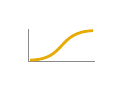
\begin{tikzpicture}[baseline=-2pt, scale=0.4]
  \draw[gtie] (0,0) -- (2.1,0);\draw[gtie] (0,0) -- (0,1.05);
  \draw[mngold, line width=1pt] (0.05,0.05) .. controls (1.2,0.05) and (0.9,0.95) .. (2.05,0.98);
\end{tikzpicture}}
% longitudinal waves: three snapshots, a spreading (gold) change over time
\newcommand{\gwaves}{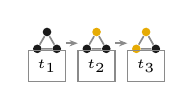
\begin{tikzpicture}[baseline=-2pt, scale=0.34]
  % frame 1
  \node[gnode] (a) at (90:0.42){};\node[gnode] (b) at (210:0.42){};\node[gnode] (c) at (330:0.42){};
  \path[gtie] (a)--(b) (b)--(c) (c)--(a);
  \node[gtie, font=\tiny] at (0,-0.85) {$t_1$};
  \path[gdir] (0.7,0) -- (1.15,0);
  % frame 2
  \begin{scope}[xshift=1.85cm]
    \node[ggnode] (a) at (90:0.42){};\node[gnode] (b) at (210:0.42){};\node[gnode] (c) at (330:0.42){};
    \path[gtie] (a)--(b) (b)--(c) (c)--(a);
    \node[gtie, font=\tiny] at (0,-0.85) {$t_2$};
    \path[gdir] (0.7,0) -- (1.15,0);
  \end{scope}
  % frame 3
  \begin{scope}[xshift=3.7cm]
    \node[ggnode] (a) at (90:0.42){};\node[ggnode] (b) at (210:0.42){};\node[gnode] (c) at (330:0.42){};
    \path[gtie] (a)--(b) (b)--(c) (c)--(a);
    \node[gtie, font=\tiny] at (0,-0.85) {$t_3$};
  \end{scope}
\end{tikzpicture}}

% ============ reusable header ============
\newcommand{\sheethead}[1]{%
\begin{tcolorbox}[enhanced, colback=mnink, colframe=mnink, arc=3pt,
  left=8pt, right=8pt, top=2pt, bottom=2pt]
\begin{minipage}[c]{0.80\textwidth}
  {\color{white}\bfseries\fontsize{18}{20}\selectfont
   Many networks \; : : \; CHEAT SHEET}\\[2pt]
  {\color{mngold}\footnotesize #1}
\end{minipage}\hfill
\begin{minipage}[c]{0.16\textwidth}\raggedleft
  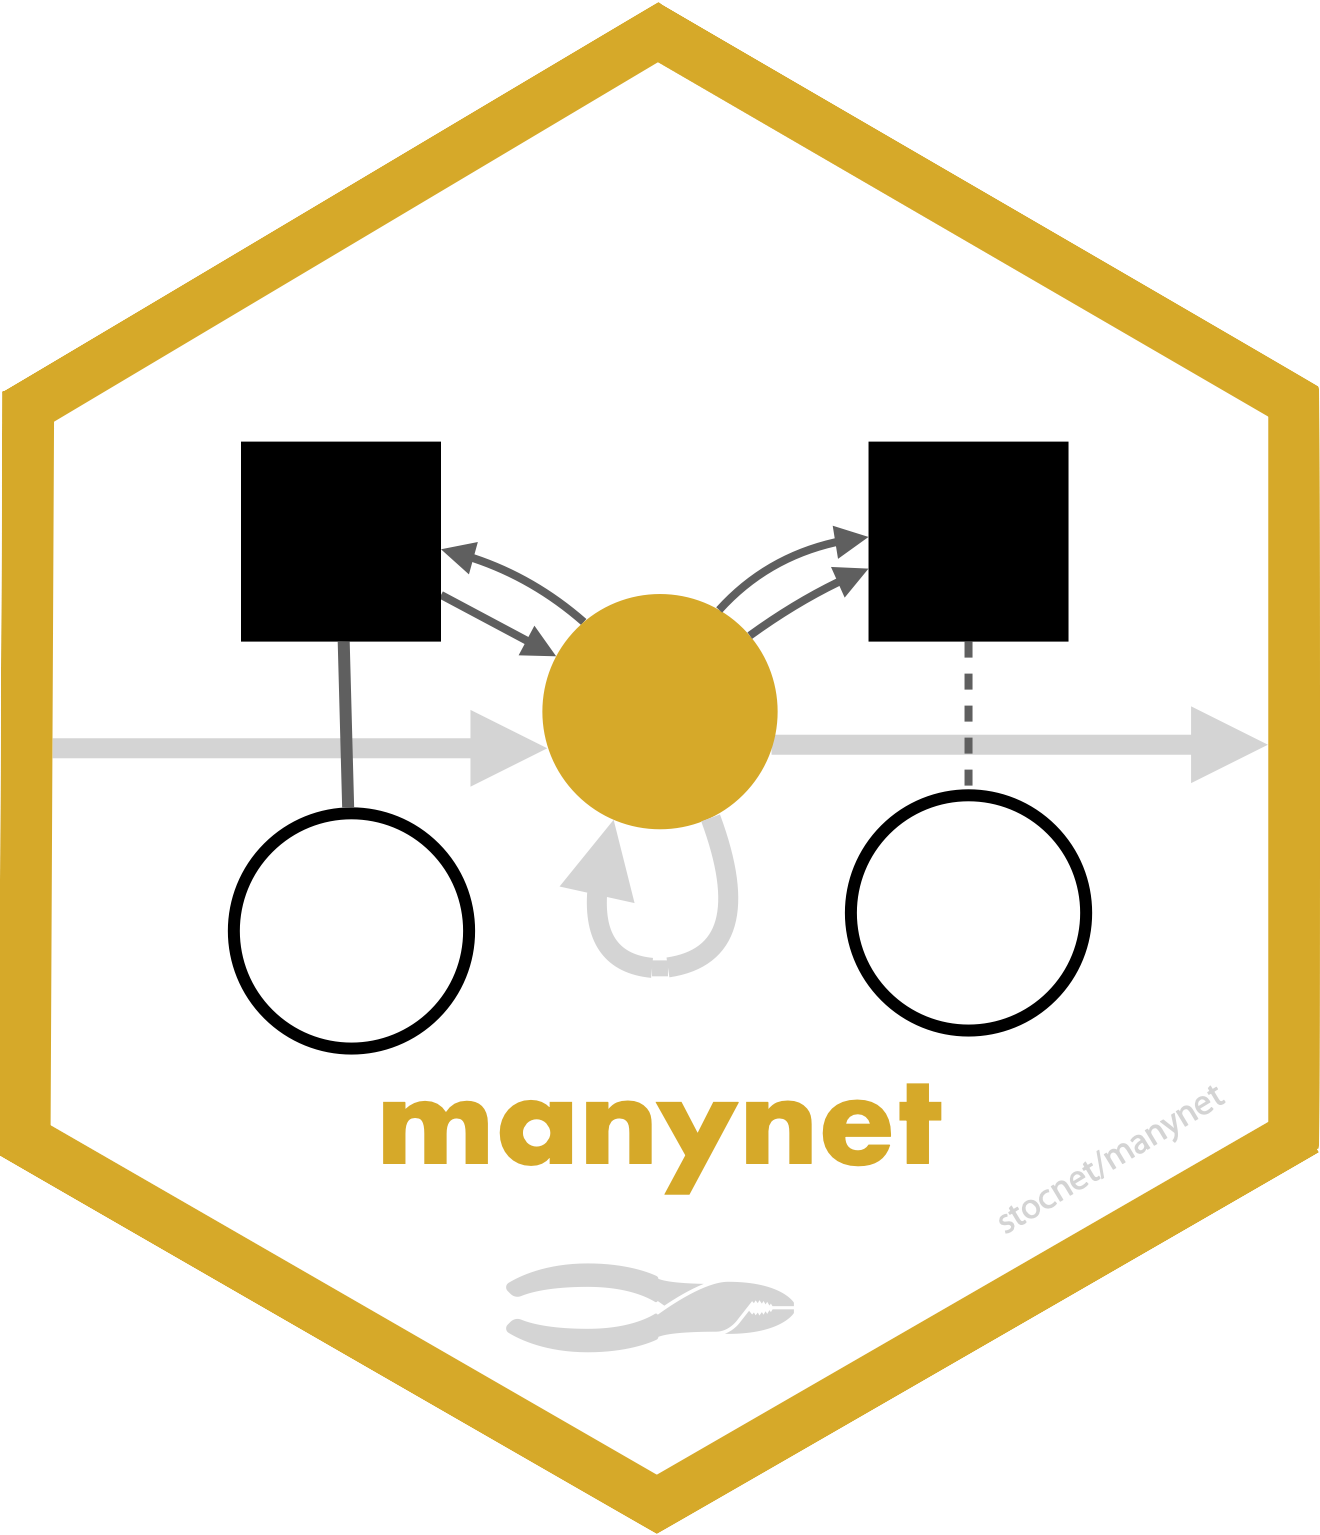
\includegraphics[height=0.58in]{logo.png}
\end{minipage}
\end{tcolorbox}}

\begin{document}

% =====================================================================
% PAGE 1 — the object + the three verbs
% =====================================================================
\sheethead{Make, manipulate, and modify many different classes, types, and formats of networks.}

% \vspace{1pt}
% 
% % ---------------- FULL-WIDTH ANATOMY ----------------
% \begin{anatbox}{Anatomy of a \texttt{stocnet}}
% \begin{minipage}[t]{0.325\textwidth}
% A \code|stocnet| is a plain list of up to five parts — built for network
% \emph{modelling} as much as analysis. Unlike the older \code|mnet| class
% (layered on \code|igraph|/\code|tbl_graph|), it holds tibbles plus rich
% metadata, carrying multimodal, multiplex, signed, longitudinal, and dynamic
% networks in one object.\\[2pt]
% \code|make_stocnet(info, nodes, ties, changes, global)| builds one;
% \code|validate_stocnet()| checks \& repairs its structure;
% \code|as_stocnet()| converts from other classes.\\[3pt]
% {\scriptsize \rchip{gold} = required \quad \chip{grey} = reserved / optional.
% Info names follow the GRAND metadata standard (FAIR-aligned).}
% \end{minipage}\hfill
% \begin{minipage}[t]{0.645\textwidth}
% \vspace{-2pt}
% \renewcommand{\arraystretch}{1.35}
% \begin{tabular}{@{}r@{\ \ }l@{}}
% \textbf{info} & \chip{name} \chip{modes} \chip{layers} \chip{directed} \chip{focal} \chip{centered} \chip{doi} \chip{date} \chip{source}\\
%  & {\scriptsize\itshape per layer:} \chip{sender} \chip{recipient} \chip{update}\\
% \textbf{nodes} & \rchip{label} \chip{mode} \chip{present} \chip{\ldots\ attributes}\\
% \textbf{ties} & \rchip{from} \rchip{to} \chip{layer} \chip{weight ($\pm$ = signed)} \chip{time} \chip{\ldots}\\
% \textbf{changes} & \rchip{node} \rchip{var} \rchip{value} \chip{time}\\
% \textbf{global} & \rchip{var} \rchip{value} \chip{time}\\
% \end{tabular}\\[3pt]
% {\scriptsize \textbf{nodes} one row per node · \textbf{ties} one row per tie ·
% \textbf{changes} logs nodal change over time · \textbf{global} logs network-level change.
% Signedness folds into \code|weight| (negative = negative tie); missing \code|weight| = missing tie.}
% \end{minipage}
% \end{anatbox}
% 
% \vspace{1pt}

% ---------------- THREE COLUMNS ----------------
\begin{minipage}[t]{0.323\textwidth}
\colhead{\faProjectDiagram}{Making networks}

\begin{mnbox}{Import \& export: \texttt{read\_*()}, \texttt{write\_*()}}
\begin{center}
files \pipe{read\_*()} \code|stocnet| \pipe{write\_*()} files
\end{center}
Formats: \code|edgelist|, \code|nodelist|, \code|matrix| (xlsx/csv),
\code|pajek|, \code|ucinet|, \code|graphml| (all read \& write);
\code|gml|, \code|gdf|, \code|dynetml| (read only).\\[2pt]
\code|read_*()| with empty parentheses opens a file browser. See also
\code|collect_cran()| for CRAN dependency networks and
\code|collect_ego()| to collect ego networks by interview prompts.
\end{mnbox}

\begin{mnbox}{Create deterministic structures}
\code|create_*()| functions always return the same structure for the same \code|n|:
\begin{center}
\renewcommand{\arraystretch}{1}
\setlength{\tabcolsep}{2pt}
\begin{tabular}{@{}ccccc@{}}
\gempty & \gfilled & \gring & \gstar & \gtree\\
{\tiny\code|empty|} & {\tiny\code|filled|} & {\tiny\code|ring|} & {\tiny\code|star|} & {\tiny\code|tree|}\\[1.5pt]
\glattice & \gcore & \gcomponents & \gwheel & \gwindmill\\
{\tiny\code|lattice|} & {\tiny\code|core|} & {\tiny\code|components|} & {\tiny\code|wheel|} & {\tiny\code|windmill|}\\
\end{tabular}
\end{center}
Also \code|create_cycle()|, \code|create_degree()|, \code|create_motifs()|, and
\code|create_explicit(A-+B)| to type out small networks by hand.
\end{mnbox}

\begin{mnbox}{Generate stochastic mechanisms}
\code|generate_*()| runs differ each time -- useful for null distributions:
\begin{itemize}
\item \code|generate_random(n, p)|: ties arise with probability \code|p|
\item \code|generate_configuration(n)|: given a degree distribution
\item \code|generate_man(n)|: given a Mutual/Asymmetric/Null dyad census
\item \code|generate_smallworld(n, p)|: ring rewired with probability \code|p|
\item \code|generate_scalefree(n, p)|: preferential attachment
\item \code|generate_fire()|, \code|generate_islands()|, \code|generate_citations()|
\end{itemize}
\textbf{Two-mode is easy}, give \code|n| two integers:
\code|create_ring(c(3,2))| \arrow \gtwomode
\end{mnbox}

\begin{mnbox}{Practice on included data}
Three families of fully documented, ready-to-analyse datasets:
\begin{itemize}
\item \code|ison_*| — classic \& instructional (\code|ison_karateka|, \ldots)
\item \code|fict_*| — fictional (\code|fict_thrones|, \code|fict_lotr|, \ldots)
\item \code|irps_*| — international politics (\code|irps_blogs|, \ldots)
\end{itemize}
\code|table_data()| gives an overview of all datasets and their formats.
\end{mnbox}

\begin{mnbox}{Describe in prose}
\code|describe_*()| functions return a readable sentence about a network,
its nodes, ties, or changes — the same summaries shown when you \code|print()| a
\code|stocnet|:
\begin{center}
\code|describe_network()|, \code|describe_nodes()|,\\
\code|describe_ties()|, \code|describe_changes()|
\end{center}
\end{mnbox}

\begin{greybox}{User interaction}
All functions operate with sensible defaults, only asking/expecting user input where necessary.

Decisions taken that affect interpretation are reported in the console.

Quieten guidance with \code|options(snet_verbosity = "quiet")|.
\end{greybox}

\end{minipage}\hfill
%
\begin{minipage}[t]{0.323\textwidth}
\colhead{\faRandom}{Manipulating networks}

\begin{mnbox}{Translate between classes: \texttt{as\_*()}}
Lossless coercion from and to many classes:
\begin{center}
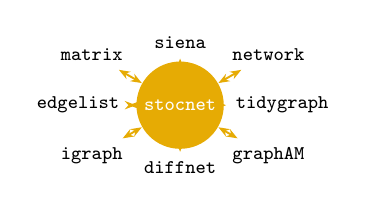
\begin{tikzpicture}[scale=0.72, font=\scriptsize\ttfamily]
  \node[circle, fill=mngold, text=white, font=\scriptsize\bfseries\ttfamily,
        inner sep=2.2pt] (c) at (0,0) {stocnet};
  \node (m) at (150:1.8) {matrix};
  \node (e) at (180:1.8) {edgelist};
  \node (i) at (210:1.8) {igraph};
  \node (n) at (30:1.8) {network};
  \node (t) at (0:1.8) {tidygraph};
  \node (g) at (-30:1.8) {graphAM};
  \node (s) at (90:1.1) {siena};
  \node (d) at (-90:1.1) {diffnet};
  \foreach \x in {m,e,i,n,t,g,s,d}{
    \path[draw=mngold, line width=0.7pt, {Stealth[length=4pt]}-{Stealth[length=4pt]}] (c) -- (\x);}
\end{tikzpicture}\\[-2pt]
\end{center}
\code|as_stocnet()|, \code|as_igraph()|, \code|as_tidygraph()|, \code|as_network()|,
\code|as_matrix()|, \code|as_edgelist()|, \code|as_siena()|, \code|as_diffnet()|.\\[2pt]
Every \code|{manynet}| function calls these coercions internally, so all
functions work on \emph{any} of these classes. Extract component tables with
\code|as_nodelist()|, \code|as_changelist()|, \code|as_infolist()|.
\end{mnbox}

\begin{mnbox}{Wrangle with a dplyr-style grammar}
Familiar verbs, suffixed by what they act on
(\code|_nodes|, \code|_ties|, \code|_changes|, \code|_globals|):

\smallskip
\begin{center}
\renewcommand{\arraystretch}{1.05}
\setlength{\tabcolsep}{3.5pt}
{\scriptsize
\begin{tabular}{@{}l|cccc@{}}
 & \code|nodes| & \code|ties| & \code|changes| & \code|globals|\\ \hline
\code|add_| / \code|delete_| & \textcolor{mngoldd}{\faCircle} & \textcolor{mngoldd}{\faCircle} & \textcolor{mngoldd}{\faCircle}\rlap{$^{d}$} & \\
\code|bind_| / \code|join_| & \textcolor{mngoldd}{\faCircle} & \textcolor{mngoldd}{\faCircle} & \textcolor{mngoldd}{\faCircle}\rlap{$^{b}$} & \\
\code|mutate_| / \code|rename_| & \textcolor{mngoldd}{\faCircle} & \textcolor{mngoldd}{\faCircle} & \textcolor{mngoldd}{\faCircle} & \textcolor{mngoldd}{\faCircle}\\
\code|filter_| / \code|select_| & \textcolor{mngoldd}{\faCircle} & \textcolor{mngoldd}{\faCircle} & \textcolor{mngoldd}{\faCircle} & \textcolor{mngoldd}{\faCircle}\rlap{$^{s}$}\\
\code|arrange_| & \textcolor{mngoldd}{\faCircle} & \textcolor{mngoldd}{\faCircle} & \textcolor{mngoldd}{\faCircle} & \\
\code|summarise_| &  & \textcolor{mngoldd}{\faCircle} &  & \\
\end{tabular}}
\end{center}
{\scriptsize $^{d}$\code|delete_| only; $^{b}$\code|bind_| only; $^{s}$\code|select_| only.}

\smallskip
E.g.\ \code|net |\code!|>!\code| mutate_ties(weight = 1) |\code!|>!\code| filter_nodes(mode == 1)|
\end{mnbox}

\begin{mnbox}{Access \& assign attributes}
Get vectors out: \code|node_names()|, \code|node_attribute(net, "x")|,
\code|tie_weights()|, \code|tie_signs()|, \code|tie_attribute(net, "y")|;
\code|mode_names()|, \code|layer_names()|.\\[1pt]
Put vectors in: \code|add_node_attribute(net, "x", vec)|, \code|add_tie_attribute()|,
or tidily via \code|mutate_nodes(net, x = vec)|.
\end{mnbox}

\begin{mnbox}{Read off metadata: \texttt{net\_*()}}
Dimensions and counts as single values:
\code|net_nodes()|, \code|net_ties()|, \code|net_dims()|,
\code|net_modes()|, \code|net_layers()|.\\[2pt]
Names of attributes present:
\code|net_node_attributes()|, \code|net_tie_attributes()|, \code|net_attributes()|,
\code|net_name()|.
\end{mnbox}

\begin{mnbox}{Mark any network: \texttt{is\_*()}}
\code|is_*()| marks return a single \code|TRUE|/\code|FALSE|:
\begin{itemize}
\item format: \code|is_directed| \code|is_weighted| \code|is_signed| \code|is_multiplex|
\code|is_twomode| \code|is_labelled| \code|is_complex| \code|is_longitudinal| \code|is_dynamic| \code|is_changing|
\item features: \code|is_connected| \code|is_acyclic| \code|is_aperiodic|
\code|is_eulerian| \code|is_perfect_matching|
\end{itemize}
Node-/tie-level variants return logical vectors, e.g. \code|node_is_mode()|,
\code|tie_is_twomode()|.
\end{mnbox}

\end{minipage}\hfill
%
\begin{minipage}[t]{0.323\textwidth}
\colhead{\faMagic}{Modifying networks}

\begin{mnbox}{Reformat: same nodes, new format}
\code|to_*()| functions work on any class and return the same class.\\[2pt]
\begin{tabular}{@{}l@{\;\;}l@{}}
\gdirected\;\code|to_directed()| & \gundirected\;\code|to_undirected()|\\
\end{tabular}\\[1pt]
also \code|to_redirected()| (swap), \code|to_reciprocated()|, \code|to_acyclic()|
\begin{itemize}
\item weights \& signs: \code|to_weighted()|, \code|to_unweighted()|,
\code|to_signed()|, \code|to_unsigned()|
\item names: \code|to_named()|, \code|to_unnamed()|;
loops \& layers: \code|to_simplex()|, \code|to_uniplex(net, tie)|
\item \code|to_anti()| — complement; \code|to_permuted()| — shuffled
\end{itemize}
\end{mnbox}

\begin{mnbox}{Transform: new dimensions}
Scope in on part of a network: \code|to_ego(net, node)|, \code|to_giant()|,
\code|to_no_isolates()|, \code|to_subgraph(net, cond)|, \code|to_blocks(net, membership)|.\\[2pt]
Keep only special tie sets: \code|to_tree()|, \code|to_matching()|, \code|to_mentoring()|,
\code|to_dominating()|, \code|to_eulerian()|.\\[2pt]
\code|to_correlation()|/\code|to_cosine()| return nodal similarity matrices.
% \emph{(See page 2 for projecting modes \& levels.)}
\end{mnbox}

\begin{mnbox}{Join \& split: \texttt{from\_*()}, \texttt{to\_*s()}}
Plural \code|to_*()| functions split a network into a list of networks, and \code|from_*()|
functions join them back up:
\begin{center}
\code|list| \pipe{from\_egos()} \code|net| \pipe{to\_egos()} \code|list|
\end{center}
\begin{itemize}
\item \code|to_egos()| / \code|from_egos()|: ego networks
\item \code|to_subgraphs(net, attr)| / \code|from_subgraphs()|
\item \code|to_components()|: one network per component
\item \code|to_waves()| / \code|from_waves()|: longitudinal panels
\item \code|to_slices(net, times)| / \code|from_slices()|: continuous time
\item \code|from_ties()|: join tie types into a multiplex network
\end{itemize}
\end{mnbox}

\begin{mnbox}{A typical pipeline}
{\ttfamily\scriptsize
ison\_southern\_women |>\\
\hspace*{1em}to\_mode1() |>\\
\hspace*{1em}mutate\_nodes(deg = netrics::node\_by\_degree(net)) |>\\
\hspace*{1em}filter\_nodes(deg > 2) |>\\
\hspace*{1em}autograph::graphr()}\\[2pt]
{\scriptsize Wrangle tidily, every step works on any class, then hand off to \code|{autograph}| /
\code|{netrics}|.}
\end{mnbox}

\begin{greybox}{The stocnet suite: Where to go next}
\begin{itemize}
\item \code|{manynet}| is for network wrangling; making, manipulating, and modifying networks\\
\item \code|{autograph}| is for network visualization; plotting and theming networks and results\\
\item \code|{netrics}| is for network analysis; marks (logical), measures (numeric), and membership (categorical)\\
\item \code|{migraph}| imports all of the above and adds some more features\\
\item \code|{RSiena}| is for longitudinal network modelling\\
\item \code|{goldfish}| is for dynamic network modelling\\
\item \code|{MoNAn}| is for mobility network modelling\\
\end{itemize}
Build a \code|stocnet| with \code|{manynet}|, then move on.
\end{greybox}

\end{minipage}

\vfill
{\scriptsize\color{mnink}
MIT License \copyright\ James Hollway \; \textbullet\;
\textbf{https://stocnet.github.io/manynet/} \; \textbullet\;
package version 2.2.0 \; \textbullet\; Updated: 2026-07
% \hfill \textbf{Page 1 of 2}: making, manipulating \& modifying}

% =====================================================================
% PAGE 2 — describing, time & levels, modelling & simulating
% =====================================================================
% \newpage
% \sheethead{Going further — describe and test networks, work across time and levels,
%    and prepare networks for modelling and simulation.}
% 
% \vspace{3pt}
% 
% \begin{minipage}[t]{0.323\textwidth}
% \colhead{\faSearch}{Describing \& testing}


% \begin{mnbox}{Handle missing data}
% Missing ties are carried as \code|NA| weights; make their treatment explicit:
% \code|na_to_zero()|, \code|na_to_mean()|, or drop incomplete nodes with
% \code|to_no_missing()|.
% Count them with \code|net_node_missing()|, \code|net_tie_missing()|.
% \end{mnbox}

% \end{minipage}\hfill
%
% \begin{minipage}[t]{0.323\textwidth}
% \colhead{\faStream}{Across time \& levels}
% 
% \begin{mnbox}{Longitudinal, dynamic \& changing}
% \code|stocnet| holds change without duplicating the whole network:
% \begin{center}\gwaves\end{center}
% \begin{itemize}
% \item \textbf{Longitudinal} (panel waves): \code|to_waves()| / \code|from_waves()|
% \item \textbf{Dynamic} (continuous time): \code|to_slices(net, times)| /
% \code|from_slices()|; \code|to_time()| snapshots at a time point
% \end{itemize}
% The \textbf{changes} table logs nodal change; work with it via
% \code|bind_changes()|, \code|mutate_changes()|, \code|filter_changes()|:
% \begin{center}
% \code|net| \pipe{gather\_changes(t)} collected \pipe{apply\_changes()} \code|net@t|
% \end{center}
% \code|gather_changes()| collects the changelog up to a time; \code|apply_changes()|
% enacts it. Test with \code|is_longitudinal()|, \code|is_dynamic()|, \code|is_changing()|.
% \end{mnbox}
% 
% \begin{mnbox}{Two-mode, multimodal \& multilevel}
% Move between levels and projections:
% \begin{center}
% \gmultilevel \pipe{to\_mode2()} \gonemode
% \end{center}
% \begin{itemize}
% \item \code|to_mode1()| / \code|to_mode2()| — project a two-mode network onto
% one node set (weighted by \code|"count"|, \code|"jaccard"|, \code|"cosine"|, \ldots)
% \item \code|to_twomode()| — split a one-mode network back into two modes
% \item \code|to_multilevel()| — stack modes as levels of one network
% \item \code|to_hypergraph()| — ties spanning $>2$ nodes
% \item \code|to_ties()| — ties become nodes (line graph)
% \end{itemize}
% Inspect with \code|net_modes()|, \code|net_layers()|,
% \code|mode_names()|, \code|layer_names()|.
% \end{mnbox}
% \end{minipage}\hfill
%
% \begin{minipage}[t]{0.323\textwidth}
% \colhead{\faFlask}{Modelling \& simulating}

% \begin{mnbox}{Model-ready metadata (\texttt{info})}
% Because \code|stocnet| keeps metadata beside the data, networks arrive ready
% to model. Reserved \code|info| names, by purpose:
% 
% \smallskip
% {\scriptsize
% \begin{tabular}{@{}p{0.24\linewidth}@{\ }p{0.70\linewidth}@{}}
% \textbf{identity} & \chip{name} \chip{doi} \chip{date} \chip{location} \chip{source}\\[3pt]
% \textbf{structure} & \chip{modes} \chip{layers} \chip{directed}\\[3pt]
% \textbf{per layer} & \chip{sender} \chip{recipient} \chip{update}\\[3pt]
% \textbf{modelling} & \chip{focal} \chip{centered} \chip{siena}\\
% \end{tabular}}
% 
% \smallskip
% \code|focal| names the dependent (endogenous) variables — tie layers and/or
% nodal behaviours; \code|centered| flags covariate centering; \code|siena| carries
% \code|{RSiena}| estimation options.\\[2pt]
% \code|as_stocnet()| / \code|as_siena()| round-trip a \code|sienadata| object
% losslessly, carrying layers, waves, covariates, and constraints across.
% \end{mnbox}

% \begin{mnbox}{Play processes over networks}
% Simulate nodal change upon any network: \hfill \gdiffusion\\[-8pt]
% \begin{itemize}
% \item \code|play_diffusion(net, seeds = 1)| — SI, SIS, SIR, SIRS, SEIR(S)
% diffusion via \code|transmissibility|, \code|recovery|, \code|waning|, \ldots
% \item \code|play_learning(net, beliefs)| — DeGroot learning until consensus
% \item \code|play_segregation(net, attribute)| — Schelling segregation
% \end{itemize}
% \code|as_diffusion()| turns empirical adoption data into comparable
% results; analyse either with \code|{netrics}| diffusion measures.
% \end{mnbox}

% \end{minipage}

% \vfill
% {\scriptsize\color{mnink}
% MIT License \copyright\ James Hollway \; \textbullet\;
% \textbf{https://stocnet.github.io/manynet/} \; \textbullet\;
% package version 2.1.5 \; \textbullet\; Updated: 2026-07
% \hfill \textbf{Page 2 of 2}: describing, time \& levels, modelling}

\end{document}
